\documentclass[]{article}
\usepackage{hyperref}
\usepackage{graphicx}
\usepackage{subfig}
\usepackage{float}

\usepackage{listings}
\usepackage{minted}
\usepackage{color}
\definecolor{dkgreen}{rgb}{0,0.6,0}
\definecolor{gray}{rgb}{0.5,0.5,0.5}
\definecolor{mauve}{rgb}{0.58,0,0.82} % or use xcolor package to choose color
\lstset{frame=tb,
	language=Python,
	aboveskip=3mm,
	belowskip=3mm,
	showstringspaces=false,
	columns=flexible,
	basicstyle={\small\ttfamily},
	numbers=none,
	numberstyle=\tiny\color{gray},
	keywordstyle=\color{blue},
	commentstyle=\color{dkgreen},
	stringstyle=\color{mauve},
	breaklines=true,
	breakatwhitespace=true,
	tabsize=3
}

\title{PJ1 Report}
\author{Chen Hao 22307110062}

\begin{document}

\maketitle

\begin{abstract}
Implementation can be found in the codes at \url{https://github.com/Laplx/DLPJ} and will also be gradually explained in the following answers. The \textit{best\_models} folder contains several model configurations, each corresponding to the specific number of question and the unsuffixed best\_model is the final selected optimal version.
\end{abstract}

\section{Question1: MLP Structure}

A full implementation of the original setting of MLP model performs normally well and has a score over 0.80.
\begin{lstlisting}
	linear_model = nn.models.Model_MLP([train_imgs.shape[-1], 600, 10], 'ReLU', [1e-4, 1e-4])
	optimizer = nn.optimizer.SGD(init_lr=0.06, model=linear_model)
	scheduler = nn.lr_scheduler.MultiStepLR(optimizer=optimizer, milestones=[800, 2400, 4000], gamma=0.5)
\end{lstlisting}

\begin{figure}
	\centering
	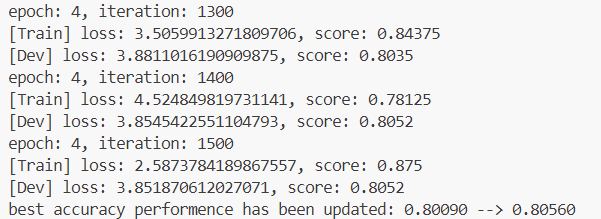
\includegraphics[width=0.7\linewidth]{Q1}
	\caption{}
	\label{fig:q1}
\end{figure}

Some modifications are:
\begin{itemize}
	\item Expand the dimension of hidden layer from 600 to 1024, which promote the accuracy slightly by enhancing the information processing.
	\begin{figure}
		\centering
		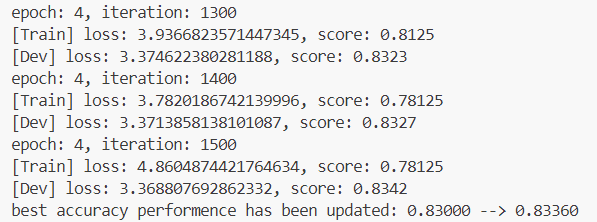
\includegraphics[width=0.7\linewidth]{Q1_2}
		\caption{}
		\label{fig:q12}
	\end{figure}
	
	\item Deepen the network shows a better result, while we also change other hyperparameters including weight\_decay and learning rate control.
	\begin{lstlisting}
		linear_model = nn.models.Model_MLP([train_imgs.shape[-1], 512, 256, 10], 'ReLU', [5e-4, 5e-4, 5e-4])
		optimizer = nn.optimizer.SGD(init_lr=0.1, model=linear_model)
		scheduler = nn.lr_scheduler.MultiStepLR(optimizer=optimizer, milestones=[300, 900, 1800], gamma=0.3)
	\end{lstlisting}
\end{itemize}
\section{Question2: Different Optimizer}

According to the momentum gradient descent, we implement MomentGD: (Note for CNN, `self.W' may be overwritten by the latter layers so distinguish them.)
\begin{lstlisting}
	class MomentGD(Optimizer):
		def __init__(self, init_lr, model, mu=0.9):
		super().__init__(init_lr, model)
		self.mu = mu
		self.v = {}
	
		# Avoid same names of params in different layers
		for layer_idx, layer in enumerate(self.model.layers):
			if layer.optimizable:
				for key in layer.params.keys():
					unique_key = f"layer{layer_idx}_{key}"
					self.v[unique_key] = np.zeros_like(layer.params[key])
			
		def step(self):
			for layer_idx, layer in enumerate(self.model.layers):
				if layer.optimizable:
					for key in layer.params.keys():
						unique_key = f"layer{layer_idx}_{key}"
						self.v[unique_key] = self.mu * self.v[unique_key] - self.init_lr * layer.grads[key]
						if layer.weight_decay:
							layer.params[key] *= (1 - self.init_lr * layer.weight_decay_lambda)
							layer.params[key] = layer.params[key] + self.v[unique_key]
						if hasattr(layer, 'sync_params'):
							layer.sync_params()
\end{lstlisting}
where we use previous settings and set \textit{batch\_size} to 64, under MomentGD, to get a score higher than 0.88.
\begin{figure}[H]
	\centering
	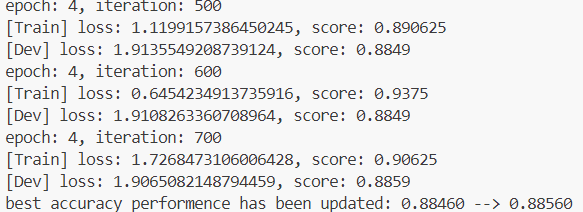
\includegraphics[width=0.7\linewidth]{Q2}
	\caption{}
	\label{fig:q2}
\end{figure}

We also exam the case when  \textit{batch\_size} is 32 and it yields a unsatisfactory outcome. The following two loss graphs show the difference clearly. (Under momentum, small batches may be too noisy to learn.)

	\begin{figure}[H]
	\centering
	\subfloat[]{
		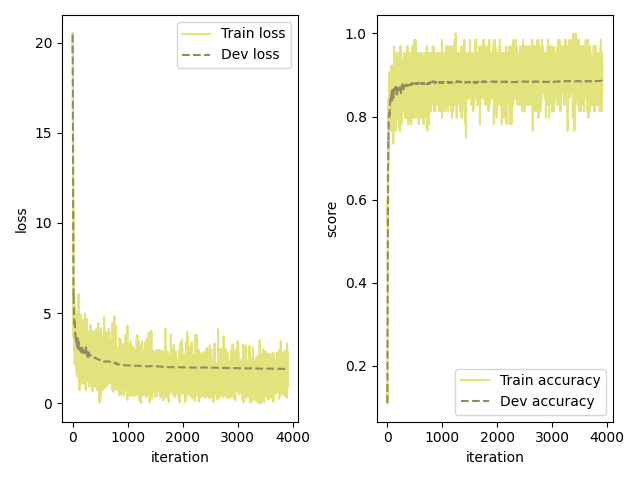
\includegraphics[width=0.45\linewidth]{Q2_a}
	}
	\hfill
	\subfloat[]{
		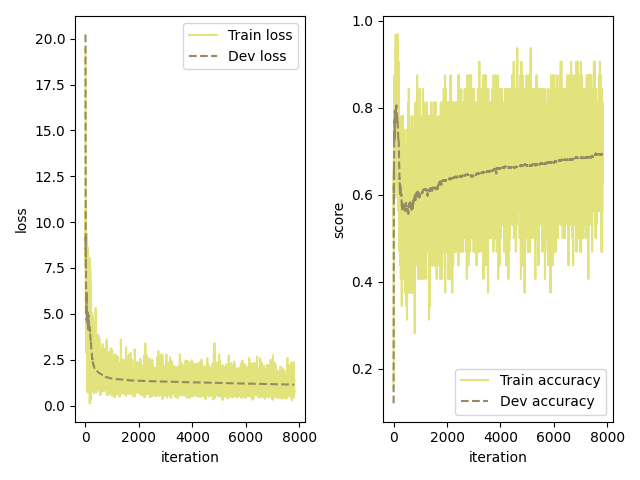
\includegraphics[width=0.45\textwidth]{Q2_b}
	}
\end{figure}

\section{Question3: Regularization}

L2 regularization(equivalent to \textit{weight\_decay}) and dropout layer has been fulfilled.

\begin{lstlisting}
class L2Regularization(Layer):
	...
	def forward(self, predicts, labels):
		loss = self.loss_fn(predicts, labels)
		for layer in self.model.layers:
		if hasattr(layer, 'weight_decay'):
			if layer.weight_decay:
				loss += np.sum(layer.W ** 2) * self.lambda_ / 2.0
	return loss

	def backward(self):
		self.loss_fn.backward()
		for layer in self.model.layers:
			if hasattr(layer, 'weight_decay'):
				if layer.weight_decay:
					layer.grads['W'] += layer.W * self.lambda_

class Dropout(Layer):
	...
	def forward(self, X):
		self.mask = np.random.binomial(1, 1-self.p, size=X.shape) / (1-self.p)
		return X * self.mask

	def backward(self, grads):
		return grads * self.mask
\end{lstlisting}

L2 penalty has already been used in the model training process and the effect of dropout method(realized by class \textit{Model\_MLP\_Dropout} that adds dropout layers after each activation functions despite the last one) see bleow(with same params). Its loss graph has the similar pattern and can be found in \textit{figs} folder.

\begin{figure}[H]
	\centering
	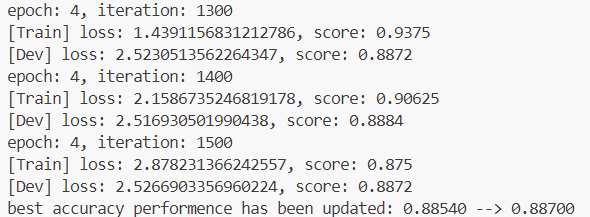
\includegraphics[width=0.7\linewidth]{Q3}
	\caption{}
	\label{fig:q3}
\end{figure}

Schedulers(MultiStepLR, ExponentialLR) are also implemented and used in the codes.

\section{Question4: Cross-Entropy Loss}

Refer to the annotation in the following codes for the calculation formulas(obtained by taking derivatives of loss function wrt. $p_{i, y_i}$).

\begin{lstlisting}
class MultiCrossEntropyLoss(Layer):
	...
	self.eps = 1e-10 # to avoid log(0)
	...
	def forward(self, predicts, labels):
		assert predicts.shape[0] == labels.shape[0], "The batch size of predicts and labels should be the same."
		assert predicts.shape[1] == self.max_classes, "The number of classes should be the same."
		self.grads = np.zeros_like(predicts)
		if self.has_softmax:
			predicts = softmax(predicts)
			self.predicts = predicts
			self.labels = labels
		
		selected_probs = predicts[np.arange(predicts.shape[0]), labels]
		loss = np.sum(-np.log(np.clip(selected_probs, self.eps, 1.0))) / predicts.shape[0]
		
		return loss
	
	def backward(self):
		batch_size = self.predicts.shape[0]
		
		if self.has_softmax:
		# Softmax + CrossEntropy: grads = (p - one_hot(labels)) / batch_size
			one_hot_labels = np.zeros_like(self.grads)
			one_hot_labels[np.arange(batch_size), self.labels] = 1
			self.grads = (self.predicts - one_hot_labels) / batch_size
		else:
		# CrossEntropy only: grads = (-1/p[labels]) / batch_size for correct class, 0 otherwise
			self.grads.fill(0)
			self.grads[np.arange(batch_size), self.labels] = -1.0 / np.clip(self.predicts[np.arange(batch_size), self.labels], self.eps, 1.0)
			self.grads /= batch_size
		
		self.model.backward(self.grads)
	
	def cancel_soft_max(self):
		self.has_softmax = False
		return self
\end{lstlisting}

\section{Question5: CNN Structure}
\begin{lstlisting}
class conv2D(Layer):
	...
	def sync_params(self):
		self.W = self.params['W']
		self.b = self.params['b']
		
	def forward(self, X):
		self.input = X
		batch_size, in_channels, H, W = X.shape

		new_H = (H - self.k_H) // self.stride + 1 #! no padding
		new_W = (W - self.k_W) // self.stride + 1
		output = np.zeros((batch_size, self.out_channels, new_H, new_W))
		
		for i in range(new_H):
			for j in range(new_W):
				output[:, :, i, j] = np.tensordot(X[:, :, i*self.stride : i*self.stride+self.k_H, j*self.stride : j*self.stride+self.k_W], self.W, axes=([1, 2, 3], [1, 2, 3])) + self.b[0, :, 0, 0] #! no padding
		
		return output
	
	def backward(self, grads):
	
		batch_size, in_channels, H, W = self.input.shape
		_, out_channels, new_H, new_W = grads.shape
		
		dW = np.zeros_like(self.W)
		db = np.zeros_like(self.b)
		dX = np.zeros_like(self.input)
		
		for i in range(new_H):
			for j in range(new_W):
				input_slice = self.input[:, :, i*self.stride : i*self.stride+self.k_H, j*self.stride : j*self.stride+self.k_W]
			
		dW += np.tensordot(grads[:, :, i, j], input_slice, axes=([0], [0]))
		db += np.sum(grads[:, :, i, j], axis=0).reshape(self.b.shape)
		dX[:, :, i*self.stride : i*self.stride+self.k_H, j*self.stride : j*self.stride+self.k_W] += np.tensordot(grads[:, :, i, j], self.W, axes=([1], [0]))
		dW /= batch_size
		db /= batch_size
		dX /= batch_size
		
		# Apply L2 regularization to dW if enabled
		if self.weight_decay:
		dW += self.weight_decay_lambda * self.W
		
		self.grads['W'] = dW
		self.grads['b'] = db
		return dX
\end{lstlisting}

Notable points here: \textit{sync\_params} to update params during optimizer.step(), avoiding losing reference. And a good way to the gradient computation is checking dimensions of all tensors at each step.

Our CNN configuartion is (only one convolution layer with out\_channel of 16, RELU between all layers):

\begin{lstlisting}
linear_model = nn.models.Model_CNN(size_list=[1, 16, 256, 10],lambda_list=[5e-4, 5e-4, 5e-4, 5e-4],kernel_size=[3, 3])
optimizer = nn.optimizer.SGD(init_lr=0.1,model=linear_model)
scheduler = nn.lr_scheduler.MultiStepLR(optimizer=optimizer,milestones=[800, 2400, 4000],gamma=0.3)
runner = nn.runner.RunnerM(linear_model, optimizer, nn.metric.accuracy, loss_fn,  batch_size=64, scheduler=scheduler)
\end{lstlisting}

Limited to the efficiency of cpu, long time is required for getting a trivial outcome. (The loss on test set decreases at first but gradually increases afterwards.)

\begin{figure}[H]
	\centering
	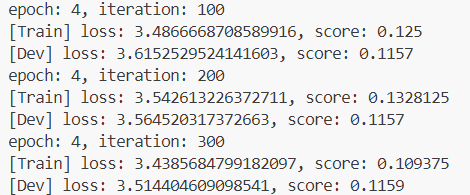
\includegraphics[width=0.7\linewidth]{Q5}
	\caption{}
	\label{fig:q5}
\end{figure}

Below is a modified CNN adding maxpool layer(kernel\_size=(2, 2), stride=2) after all convolution layers, which raises the best score up to 0.37. Bottleneck structure is also implemented in the codes.

\begin{figure}[H]
	\centering
	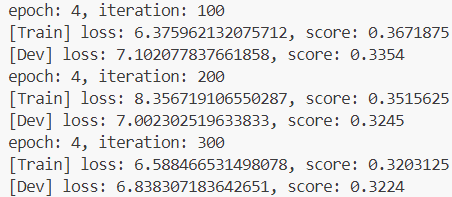
\includegraphics[width=0.7\linewidth]{Q5_2}
	\caption{}
	\label{fig:q52}
\end{figure}

\section{Question6: Data Augmentation}
We adopt a variety of tranformation including shift, rotation and scale.

\begin{lstlisting}
	def augment_images(images, labels, num_augmentations=2):
		augmented_images = []
		augmented_labels = []
		
		for img, label in zip(images, labels):
			img_2d = img.reshape(28, 28)
		
			augmented_images.append(img)
			augmented_labels.append(label)
			
			for _ in range(num_augmentations):
				shift_x = np.random.uniform(-2, 2)
				shift_y = np.random.uniform(-2, 2)
				shifted_img = shift(img_2d, [shift_y, shift_x], mode='nearest')
				
				angle = np.random.uniform(-10, 10)
				rotated_img = rotate(shifted_img, angle, reshape=False, mode='nearest')
				
				scale = np.random.uniform(0.9, 1.1)
				scaled_img = zoom(rotated_img, scale, mode='nearest')
				
				if scaled_img.shape != (28, 28):
					scaled_img = zoom(scaled_img, (28 / scaled_img.shape[0], 28 / scaled_img.shape[1]), mode='nearest')
					
				augmented_images.append(scaled_img.flatten())
				augmented_labels.append(label)
		
		return np.array(augmented_images), np.array(augmented_labels)
\end{lstlisting}

with the following typical setting:
\begin{lstlisting}
	linear_model = nn.models.Model_MLP([train_imgs.shape[-1], 512, 256, 10], 'ReLU', [5e-4, 5e-4, 5e-4])
	optimizer = nn.optimizer.MomentGD(init_lr=0.1, model=linear_model, mu=0.9)
	scheduler = nn.lr_scheduler.MultiStepLR(optimizer=optimizer, milestones=[300, 900, 1800], gamma=0.3)
	loss_fn = nn.op.MultiCrossEntropyLoss(model=linear_model, max_classes=train_labs.max()+1)
	runner = nn.runner.RunnerM(linear_model, optimizer, nn.metric.accuracy, loss_fn, batch_size=64, scheduler=scheduler)
\end{lstlisting}
\begin{figure}[H]
	\centering
	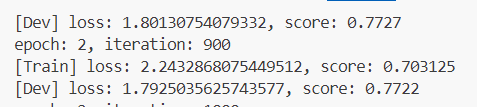
\includegraphics[width=0.7\linewidth]{Q6}
	\caption{}
	\label{fig:q6}
\end{figure}

SGD yields a probably worse result since it was ​​stuck in a local optimum​.

\begin{figure}[H]
	\centering
	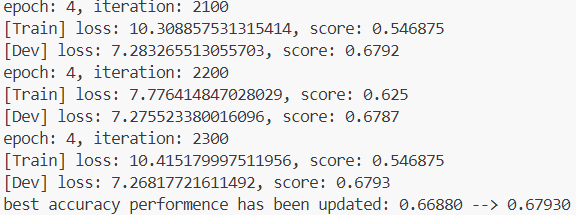
\includegraphics[width=0.7\linewidth]{Q6_2}
	\caption{}
	\label{fig:q62}
\end{figure}

\section{Question7: Visualization of Kernel Weights}
Rewrite visualization code in \textit{weight\_visualization.py} and get the following result for CNN implemented in Sec.5.

\begin{figure}[H]
	\centering
	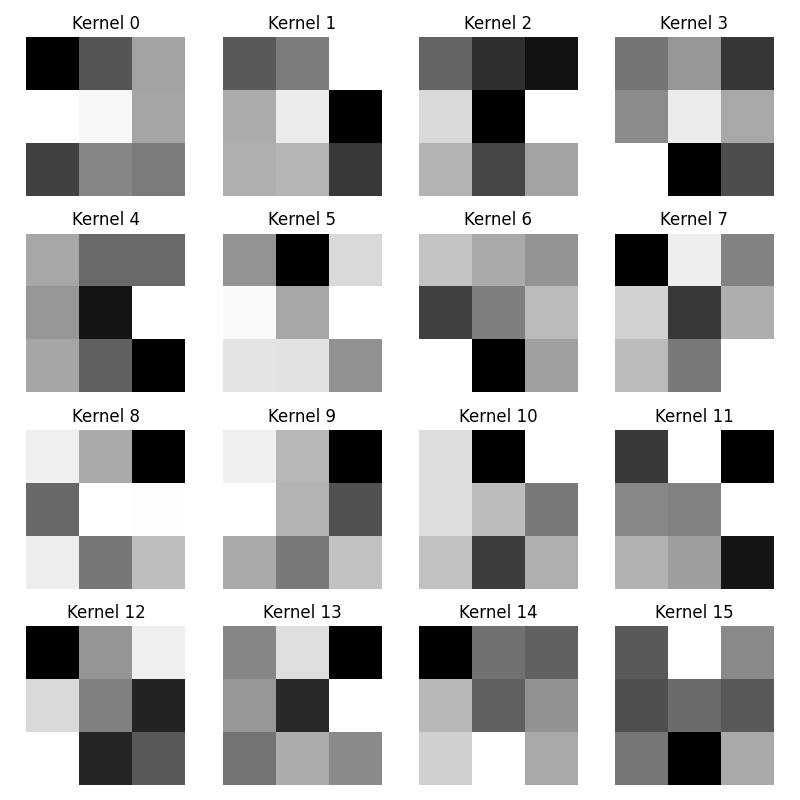
\includegraphics[width=0.55\linewidth]{kernels}
	\caption{}
	\label{fig:kernels}
\end{figure}

Here we can discover some patterns in writing strokes of numbers.

\end{document}
